\documentclass{article}

\usepackage{tikz}
\usetikzlibrary{calc,fit,shapes,arrows}

\usepackage{listings}

\newcommand{\informed}[0]{{\sc informed}}

\title{Stopwatch architecture design using \informed}


\lstdefinelanguage{SPARK}{
  language = [95]Ada,
  morekeywords = {pre,post,assert,assume,check,derives,hide,global,inherit,from,own,initializes,main_program},
  comment=[l][commentstyle]{--\ },
  texcl=true,
  showstringspaces=false
}

\lstdefinestyle{tinystyle}
   {basicstyle=\footnotesize\tt,
    keywordstyle=\color{blue},
    commentstyle=\rmfamily\it\color{gray},
    captionpos=b,
    caption={},label={},
    numbers=none,
    escapeinside={(*}{*)}}

\lstset{language=SPARK}
\lstset{style=tinystyle}


\tikzstyle{main}=[regular polygon,
                  regular polygon sides=3,
                  draw,
                  minimum width=1cm,
                  inner sep=0.05cm,
                  text badly centered,
                  font=\scriptsize]
\tikzstyle{var}=[draw,
                 text badly centered,
                 text width=1cm,
                 font=\scriptsize]
\tikzstyle{type}=[rectangle,
                  draw,
                  rounded corners,
                  minimum width=1cm,
                  minimum height=0.5cm,
                  text badly centered,
                  font=\scriptsize]
\tikzstyle{boundary}=[single arrow,
                      draw,
                      shape border rotate=270,
                      single arrow head extend=0.0cm,
                      minimum height=0.75cm,
                      minimum width=0.75cm,
                      single arrow tip angle=120,
                      text badly centered,
                      text width=0.75cm,
                      font=\scriptsize]
\tikzstyle{utility}=[trapezium,
                     trapezium left angle=100,
                     trapezium right angle=100,
                     draw,
                     minimum width=.75cm,
                     minimum height=0.5cm,
                     inner sep=0.01cm,
                     minimum height=0.5cm,
                     text badly centered,
                     font=\scriptsize]

\tikzstyle{strong}=[-triangle 90]
\tikzstyle{weak}=[-open triangle 90]

\makeatletter
\renewcommand\paragraph{\@startsection{paragraph}{4}{\z@}%
                                    {3.25ex \@plus1ex \@minus.2ex}%
                                    {-1em}%
                                    {\normalfont\normalsize\itshape}}
\makeatother


\begin{document}

\section{Introduction}
\label{Introduction}
Software Engineering is concerned with the controlled and correct development of Systems(Machines) that impact upon the environment in which they are deployed (World). Where the objective of the deployment of a Machine is to improve the World.
 
\paragraph{}The purpose of Requirements Engineering is to take a set of Stakeholder Requirements and arrive at a complete, correct and usable set of System Specification Statements for the system under development. Within REVEAL\texttrademark the application of the process is also intended to have a wider objective of adding benefits to the project Stakeholders through learning, negotiation and the development of trust between all parties involved in the production of the system.

\paragraph{}REVEAL\texttrademark is Altrans' systematic method for the elicitation, specification and management of System Requirements. Through its application we clearly identify three key artefacts:

	\begin{itemize}
           \item Requirements (R) which are statements about things in the World that we want the System to make true.
           \item Specification Statements(S) describe the Systems external behaviour. 
   	   \begin{itemize}
             \item Specifications include only shared phenomena in the interface between the World and the System being developed.
             \item Specifications can only constrain shared phenomena that the System can control.
           \end{itemize}
           \item Domain Statements(D) which are knowledge about the World, that is generally assumed and not normally documented, but must hold if the Specification Statements are to fully satisfy the System Requirements.
         \end{itemize}

\paragraph{}Once this information has been gathered, a Satisfaction Argument is constructed to show that all the Stakeholder Requirements have been addressed through the System Specification and Domain Statements. (As Verification and Validation progresses, V\&V Plans and summary results can also inform the satisfaction argument, although this may not be done for the competition.) 

\paragraph{}The REVEAL\texttrademark process is far more extensive than that described above including detailed processes for:
	\begin{itemize}
          \item Stakeholder Identification, 
          \item Knowledge Elicitation, 
          \item Requirement Verification and Validation,
          \item Conflict Management and Resolution,
          \item Requirements Maintenance and Management.
        \end{itemize}

\paragraph{}More information on the REVEAL method can be found on \url{http://intelligent-systems.altran.com/technologies/systems-engineering/revealtm.html}.

\paragraph{}Since by its nature the VSTTE 2013 competition has a very short timescale, and the Requirements are provided by the competition organisers it is not expected that there would be time to apply a full REVEAL\texttrademark process, however the benefits of Requirements capture, expression, satisfaction arguments and traceability can be shown by their application in this context.



\section{Diagram}

\begin{figure}[h]
  \begin{center}
    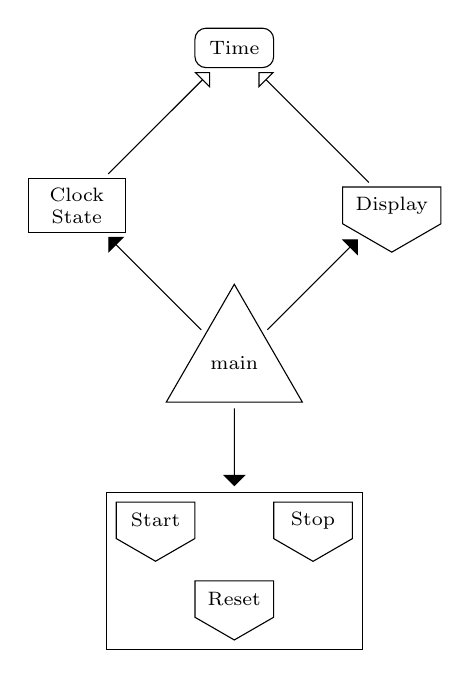
\begin{tikzpicture}[x=2cm,y=2cm,shorten >=2pt, shorten <=2pt]
      \node[main] (main) at (0, 0) {main};

      \node[var] (clock_state)                  at (-1, 1) {Clock\\State};
      \node[boundary, text width=1cm] (display) at ( 1, 1) {Display};
      \node[type]     (time)                    at ( 0, 2) {Time};

      \node[boundary] (start)       at (-0.5, -1) {Start};
      \node[boundary] (stop)        at ( 0.5, -1) {Stop};
      \node[boundary] (reset)       at ( 0, -1.5) {Reset};

      \node[draw, fit=(start) (stop) (reset)] (buttons) {};

      \draw[->,strong] (main) -- (clock_state);
      \draw[->,strong] (main) -- (display);
      \draw[->,weak] (clock_state) -- (time);
      \draw[->,weak] (display) -- (time);
      \draw[->,strong] (main) -- (buttons);
    \end{tikzpicture}
  \end{center}
  \caption{\informed\ diagram of our Stopwatch}
\end{figure}

\pagebreak
\section{\informed\ package structure}

\subsection{Time}
\lstinputlisting{spark/time.ads}

\subsection{Clock State}
\lstinputlisting{spark/clock.ads}

\subsection{Display}
\lstinputlisting{spark/display.ads}

\subsection{Controls}
\lstinputlisting{spark/controls.ads}

\subsection{Main}
\lstinputlisting{spark/main.adb}

\appendix
\section{\informed\ Element Definitions}

\subsection{\informed\ Main Program}

\begin{wrapfigure}{l}{1.75cm}
  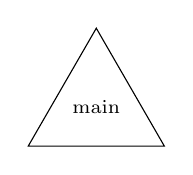
\begin{tikzpicture}
    \node[main] at (0, 0) {main};
  \end{tikzpicture}
\end{wrapfigure}
This section show you how an \informed\ Main Program is represented
pictorially on an architecture diagram, and as a SPARK package.

Typically, the SPARK implementation of an \informed\ design will have
only one such main program (annotated with SPARK's
\texttt{main\textunderscore program} annotation).

\begin{lstlisting}[caption=An \informed\ SPARK Main program]
with A, B, C, D;

procedure Main
  with Global => (Input => (I1, I2, I3),
                  Output => (O1, O2))
is
begin  -- Main
   Initialize;
   loop
      ControlProcedure;
   end loop;
end Main;
\end{lstlisting}


\subsection{\informed\ Variable Packages}

\begin{wrapfigure}{l}{1.5cm}
    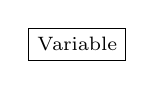
\begin{tikzpicture}
      \node[var] at (0, 0) {Variable};
    \end{tikzpicture}
\end{wrapfigure}

This section show you how an \informed\ Variable Package is
represented pictorially on an architecture diagram, and as a SPARK
package.

Rather than provide a generic example, this section uses a Stack
package to provides a concrete example of an \informed\ variable
package. In this example we are defining a container
(\texttt{Stack.State}) that can contain values of a certain shape
("abstract stack") upon which certain operations can be performed
(\texttt{Clear}, \texttt{Push} and \texttt{Pop}).


\begin{lstlisting}[caption=An \informed\ SPARK variable package]
package Stack
  with Abstract_State => State
is

  procedure Clear;
    with Global => (Output => State);

  procedure Push(X : in Integer);
    with Global => (In_Out => State);

  procedure Pop(X : out Integer);
    with Global => (In_Out => State);

end Stack;
\end{lstlisting}

\subsection{\informed\ Type Packages}

\begin{wrapfigure}{l}{1.5cm}
  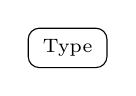
\begin{tikzpicture}
    \node[type] at (0, 0) {Type};
  \end{tikzpicture}
\end{wrapfigure}

This section show you how an \informed\ Type Package is represented
pictorially on an architecture diagram, and as a SPARK package. This
type of package does not have a state and therefore does not require a
State declaration, and this is shown in the code below.

The stack variable package presented earlier can be restructured as a
type package declaring an abstract type.

\begin{lstlisting}[caption=An \informed\ SPARK Type Package]
package Stack is

  type T is private;

  procedure Clear (S : out T);

  procedure Push (X : in     Integer;
                  S : in out T);

  procedure Pop (X : out    Integer;
                 S : in out T);

private

  -- full declaration of type T would go here

end Stack;
\end{lstlisting}


\subsection{\informed\ Utility Packages}

\begin{wrapfigure}{l}{1.75cm}
  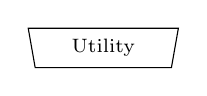
\begin{tikzpicture}
    \node[utility] at (0, 0) {Utility};
  \end{tikzpicture}
\end{wrapfigure}

This section show you how an \informed\ Utility Package is represented
pictorially on an architecture diagram. No example of a SPARK Utility
package is provided here since these are of such a general nature.

However, care should be taken when implementing an \informed\ design
as it is easy for there to be an excessive proliferation of
packages. In many cases the correct place for an operation is in the
type or variable pacakage upon which it operates. The key thing for an
\informed\ design is for the operations to be correctly located.

\subsection{\informed\ Boundary Variable Packages}
\begin{wrapfigure}{l}{1.75cm}
  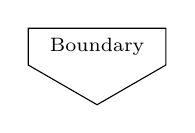
\begin{tikzpicture}
    \node[boundary,text width=1.5cm] at (0, 0) {Boundary};
  \end{tikzpicture}
\end{wrapfigure}

This section show you how an \informed\ Boundary Variable Package is
represented pictorially on an architecture diagram, and as a SPARK
package.

A boundary variable is a variable package; however, unlike other
instances of such variables the name provided in its own variable
clause is a place holder representing the stream of data arriving
from, or being sent tom the outside world rather than simply an
abstract name for the internal state of the package.

It is often useful to place an abstraction layer between the boundary
variables of a system and their users; this approach is appropriate
where direct use of the boundary variables would provide insufficient
abstraction allowing too much detail to become visable in higher level
SPARK annotations. An example of this abstraction layer is include in
the code example shown below.

\begin{lstlisting}[caption=An \informed\ SPARK Boundary Variable Package]
package Controls
  with Abstract_State => (Start, Stop, Reset)
is

  procedure Read_Start_State (Is_Pressed : out Boolean)
    with Global => (Input => Start);

  procedure Read_Stop_State (Is_Pressed : out Boolean)
    with Global => (Input => Stop);

  procedure Read_Reset_State (Is_Pressed : out Boolean)
    with Global => (Input => Reset);

end Controls;

with Controls;
private package Controls.Reset
   with Abstract_State => (Reset)
is
  procedure Read (Is_Pressed : out Boolean)
    with Global => (Input => Reset);
end Controls.Reset;

with Controls;
private package Controls.Start
   with Abstract_State => (Start)
is
  procedure Read (Is_Pressed : out Boolean)
    with Global => (Input => Start);
end Controls.Start;

with Controls;
private package Controls.Stop
   with Abstract_State => (Stop)
is
  procedure Read (Is_Pressed : out Boolean)
    with Global => (Input => Stop);
end Controls.Stop;

\end{lstlisting}

\subsection{\informed\ Connectors}

\begin{wrapfigure}{l}{1.75cm}
  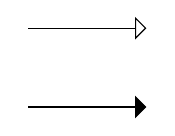
\begin{tikzpicture}
    \draw[->,strong] (0, 0) -- (1.5, 0);
    \draw[->,weak]   (0, 1) -- (1.5, 1);
  \end{tikzpicture}
\end{wrapfigure}

Descriptive Text...


\end{document}
